% !TeX spellcheck = en_US
\chapter{The proposed decentralized solution}\label{cha:decentralizedSystem}

This chapter describes the proposed decentralized solution created to address the four problems presented in the problem statement (\cref{sec:problemStatement}). The expectation is that the decentralized solution will perform better than the centralized solution (presented in \cref{cha:existingSystem}) on the following parameters:

\begin{description}
	\item[Scalability] in terms of turbines per Park Pilot.
	In the current Siemens system the number of turbines is effectively limited by the maximum length of the regulation cycle time.
	The length of the regulation cycle time is decided by time of retrieving each turbine's state, added to the time required to calculate new setpoints, added to the time of distributing new setpoints to each turbine. Adding turbines to the Park Pilot will prolong the regulation cycle of retrieving turbine states, calculation of new setpoints and distribution of the new setpoints. As the regulation cycle time is not allowed to increase indefinitely the number of turbines of one Park Pilot must be limited such that the regulation cycle time does not exceed it's maximum length.
	The theory is that decentralizing the Park Pilot will enable a more dynamic system, where increasing the number of turbines also increases the resources (in terms of computational power and memory) available to the system. Increasing the number of nodes in a decentralized system will increase the network traffic of the system, which can be a problem as the network will congest given enough connected nodes. Siemens has informed that the current Siemens system operates on a gigabit network, making bandwidth a minor issue, but an issue that has to be solved at some point nevertheless. Even if this issue presents itself, one could imagine a decentralized system where the turbines are automatically clustered, such that communication in the network is limited to full communication within clusters and generel communication between clusters.
	\item[Availability] in terms of fault tolerance. Decentralizing the Park Pilot out on the turbines removes the Park Pilot as a single point of failure. Thus the decentralized solution will no longer be vulnerable to failures in the Park Pilot as it is decentralized across turbines.
	\item[Performance] in terms of regulation cycle time. In the decentralized solution a turbine will proactively distribute it's own calculated state as soon as it is available, thus avoiding the request/reply approach of the current Siemens system. The need to request data as the first step of the regulation cycle is thus alleviated, decreasing the overall time of the regulation cycle. When state is shared between turbines proactively every turbine has enough information locally to calculate it's own setpoint. The calculation of setpoints is thus removed from the Park Pilot and distributed into each individual turbine. 
\end{description}


\noindent The decentralized solution is built using the knowledge of the current Siemens system, obtained when developing the centralized solution. Changes made from the centralized solution to the decentralized solution are only specific to the change in the architecture when decentralizing the system. QoS parameters differ only in the parameters that interfere with the decentralized implementation. The wind data sent and received is the same for both systems.

%This chapter describes the decentralized solution by first describing what decentralizing the system means to the regulation algorithm. Furthermore the chapter describing the decentralized solution through a detailed description of the regulation cycle of the decentralized solution, followed by a description of the DDS QoS parameters used.
First the changes to the regulation algorithm to make it compatible with a decentralized architecture is described, then the DDS QoS parameters of the decentralized solution is presented.

\section{Regulation algorithm}

Decentralizing the regulation algorithm from the centralized solution (\cref{sec:cenRegAlgorithm}), we get the input/outputs presented in \cref{fig:ioDecenRegAlg}.

\begin{figure}[!h]
	\centering
	\begin{tikzpicture}[
	point/.style={inner sep=0pt}, %circle,minimum size=2pt,fill=red},
	textNode/.style={inner sep=2pt},
	hv path/.style={to path={-| (\tikztotarget)}},
	vh path/.style={to path={|- (\tikztotarget)}},
	skip loop h/.style={to path={-- ++(0,#1) -| (\tikztotarget)}},
	skip loop v/.style={to path={-- ++(#1,0) |- (\tikztotarget)}},
	graphs/every graph/.style={edges=rounded corners}
	]
	
% Place nodes
\matrix[row sep=1.5cm,column sep=.5cm] {
	\node [point]  		(p1x1)	{}; &&
	\node [rectangle]	(Turbine)		[draw, label=above:Turbine, text width=50pt]	{Cur.prod. Max.prod}; &&
	\node [point]  		(p1x3)	{}; \\
	
	\node [point]  		(p2x1)			{}; &&
	\node [textNode]	(HPPP)		 	{Reg.algorithm}; &&
	\node [textNode]	(Setpoint)	{Setpoint}; \\

	\node [textNode]  (gSetpoint)										{Global setpoint}; &&
	\node [rectangle]	(Data)			[draw, text width=50pt] {Cur.prod  Max.prod};\\
};

\node [textNode,right of=Data] {~~~~~~~~~~~~~~~~~\textbf{$\cdot$}nTurbines-1};
	
\graph[use existing nodes]{
	Turbine ->[skip loop v=-3.1cm] HPPP -> Setpoint ->[vh path] Turbine;
	gSetpoint.east -> HPPP;
	Data -> HPPP;
};

\end{tikzpicture}

	\captionsetup{format=plain,font=footnotesize,labelfont={bf,defaultCapFont},labelsep=quad,singlelinecheck=no}
	\caption[Decentralized input/output parameters of the regulation algorithm]{
		\label{fig:ioDecenRegAlg} 
		\footnotesize{%
			Decentralized input/output parameters of the regulation algorithm.
		}
	}
\end{figure}

The regulation algorithm is now computed on every turbine instead of computing the algorithm on a central Park Pilot. Thus, instead of requesting all states (current production and max production) externally, the regulation algorithm now collects one state from the local turbine. Furthermore the regulation algorithm only calculates a single setpoint - the setpoint used by the local turbine to set a new state - instead of calculating a setpoint for every turbine in the wind farm.

As \cref{fig:ioDecenRegAlg} implies, with the regulation algorithm performed on every turbine, decentralizing the Park Pilot onto the turbines also means that every turbine must know the state of every other turbine in the wind farm.

\section{Regulation cycle}

Decentralizing the Park Pilot onto the turbines has changed the regulation cycle too. The decentralized solution has been built with focus on scalability, in terms of increasing the number of turbines does not impact the regulation cycle, as well as performance, in terms of decreasing the regulation cycle time.

The following sections presents the decentralized regulation cycle. First by describing how the decentralized regulation cycle differs from the centralized regulation cycle, followed by a detailed description of how a single regulation cycle has been implemented. 

%Finally the term \textit{cache reads} is discussed, which is introduced by the decentralized by a discussion of the introduction of cache reads.

\subsection{Changes compared to the centralized regulation cycle}\label{sec:regCycleChanges}

The difference between the centralized regulation cycle and the decentralized regulation cycle is illustrated in \cref{fig:cycleCentralVSDecentral}. 

\begin{figure}[!h]
	%The figure show how regulation time differs central vs decantral

	{\sffamily{Centralized regulation cycle}}
	\newline
	

{ %The brackets issolate the enviroment

\tikzstyle{line}		 	= [draw]

\makeatletter
\ifcsname c@wavenum\endcsname %Only create one counter
\else
	\newcounter{wavenum}
\fi
\makeatother

\newcommand*{\bitvector}[3]{
  \draw[fill=#3] (t_cur) -- ++( .1, .3) -- ++(#2-.2,0) -- ++(.1, -.3)
                         -- ++(-.1,-.3) -- ++(.2-#2,0) -- cycle;
  \path (t_cur) -- node[anchor=mid](textNode) {#1} ++(#2,0) node[time] (t_cur) {};
  }

% \known{val}{length}
\newcommand*{\known}[2]{
    \bitvector{#1}{#2}{white}
}

% \unknown{length}
\newcommand*{\unknown}[2]{
    \bitvector{#1}{#2}{black!20}
}

% \nextwave{name}
\newcommand{\nextwave}[1]{
  %\path (0,\value{wavenum}) node[time] (t_cur) {};
   \path (0,\value{wavenum}) node[left] {#1} node[time] (t_cur) {};
  \addtocounter{wavenum}{-1}
}

\newcommand{\timeSpanLabel}{
	\node (CycleTimeLabel) [rectangle, above = 0.7cm of textNode, inner sep=0pt] {Regulation cycle time};	  
}

\newcommand{\timeSpanA}{
	\node (t_timeSpanA) [point, above = 0 of t_cur] {};	  
}

\newcommand{\timeSpanB}{
	\node (t_timeSpanB) [point, above =0 of t_cur] {};

  \graph[use existing nodes]{
  	t_timeSpanA --[time span=1cm] CycleTimeLabel;
   	CycleTimeLabel.south --[time span=-0.24cm] t_timeSpanB;
  }; 
    	
}


%%% End of timing.sty
\begin{tikzpicture}[
	point/.style={inner sep=0pt}, %circle,minimum size=2pt,fill=red},
	draw=black, 
	yscale=.8,
	xscale=1,
	hv path/.style={to path={-| (\tikztotarget)}},
	vh path/.style={to path={|- (\tikztotarget)}},
	skip loop v/.style={to path={-- ++(#1,0) |- (\tikztotarget)}},		
	skip loop h/.style={to path={-- ++(0,#1) -| (\tikztotarget)}},
	time span/.style={to path={-- ++(0,#1) -| (\tikztotarget)}},
	graphs/every graph/.style={edges=rounded corners}	
	]
	
  \tikzstyle{time}=[coordinate]
  \setlength{\unitlength}{1cm}
  \setcounter{wavenum}{0}
    
  %\nextwave{Regulation Time} \unknown{SendData}{2} \known{WaitForData}{5} \unknown{ReciveData}{2} \unknown{Calculate}{2}\unknown{SendSP}{2}
  \nextwave{Park Pilot} \unknown{reqStates}{1.8} \known{wait}{2} \unknown{readStates}{2} \unknown{regAlg.}{1.7} \unknown{sendSetpoints}{2.6}
  
  \nextwave{Turbine} \known{wait}{1.8} \unknown{replyState}{2} \known{wait}{6.3} \unknown{receiveSetpoint}{2.9}
    
  
\end{tikzpicture}
}

	\newline
	
	{\sffamily{Decentralized regulation cycle (with parallel reception of data)}}
	\newline
	

{ %The brackets issolate the enviroment

\makeatletter
\ifcsname c@wavenum\endcsname %Only create one counter
\else
	\newcounter{wavenum}
\fi
\makeatother

\newcommand*{\bitvector}[3]{
  \draw[fill=#3] (t_cur) -- ++( .1, .3) -- ++(#2-.2,0) -- ++(.1, -.3)
                         -- ++(-.1,-.3) -- ++(.2-#2,0) -- cycle;
  \path (t_cur) -- node[anchor=mid](textNode) {#1} ++(#2,0) node[time] (t_cur) {};
}

% \known{val}{length}
\newcommand*{\known}[2]{
    \bitvector{#1}{#2}{white}
}

% \unknown{length}
\newcommand*{\unknown}[2]{
    \bitvector{#1}{#2}{black!20}
}

% \nextwave{name}
\newcommand{\nextwave}[1]{
  %\path (0,\value{wavenum}) node[left] {#1} node[time] (t_cur) {};
  %\path (0,\value{wavenum}) node[time] (t_cur) {};
  \path (0,\value{wavenum}) node[below left] {#1} node[time] (t_cur) {};
  \addtocounter{wavenum}{-1}
}


\newcommand{\timeSpanA}{
	\node (t_timeSpanA) [point, above = 0 of t_cur] {};	  
}

\newcommand{\timeSpanB}{
	\node (t_timeSpanB) [point, above =0 of t_cur] {};
	
	\graph[use existing nodes]{
		t_timeSpanA --[time span=1cm] CycleTimeLabel;
		CycleTimeLabel.south --[time span=-0.24cm] t_timeSpanB;
	}; 
	
}

%%% End of timing.sty

\begin{tikzpicture}[
	point/.style={inner sep=0pt}, %circle,minimum size=2pt,fill=red},
	draw=black, 
	yscale=.8,
	xscale=1,
	hv path/.style={to path={-| (\tikztotarget)}},
	vh path/.style={to path={|- (\tikztotarget)}},
	skip loop v/.style={to path={-- ++(#1,0) |- (\tikztotarget)}},		
	skip loop h/.style={to path={-- ++(0,#1) -| (\tikztotarget)}},
	time span/.style={to path={-- ++(0,#1) -| (\tikztotarget)}},
	graphs/every graph/.style={edges=rounded corners}	
]
	
\tikzstyle{time}=[coordinate]
\setlength{\unitlength}{1cm}
\setcounter{wavenum}{0}

	\nextwave{Turbine} \unknown{readStates}{2.5} \unknown{regAlg.}{2.5} \unknown{setSetpoint}{2.5} \unknown{sendState}{2.5} \known{sleep}{2}
	\nextwave{} \known{reciveStates}{12}
\end{tikzpicture}
}

	\caption{Centralized vs decentralized regulation cycle}
	\label{fig:cycleCentralVSDecentral}
\end{figure}

In the centralized solution a request for data and waiting for the corresponding reply for every turbine was a requirement for the Park Pilot, turbines in the decentralized solution publish new states whenever a new setpoint has been calculated. Turbines publishes to a specific Topic and are assigned a unique keys. Receiving states from other turbines is handled and loaded asynchronously into memory by Connext, thus receiving states is a parallel process running alongside the regulation algorithm.
This enables a \textit{Distributed Shared Memory (DSM)} (see \cref{sec:DSM} for DSM description) behavior for the decentralized solution, where the state of every turbine is shared with every other turbine in the wind farm.
As every turbine has a unique Topic key, each turbine has assigned its own shared memory space, where only the turbine is allowed to write, as illustrated in \cref{fig:DSMlikeBehavior}, thus removing the possibility that turbines overwrite each others states. Using DSM like behavior for the decentralized solution, means that receiving states from other turbines is abstracted away from the regulation cycle, enabling the turbines to assume that the latest state of every other turbine has been received and is available locally in memory. This alleviates the need for the request-reply part of the centralized regulation cycle. The expectation is that removing the request-reply part of the algorithm decreases the regulation cycle time, since acquisition of turbine states are no longer a part of the regulation cycle.  

\begin{figure}[!h]
	\begin{tabular}{ | c | c | c | c | c |}
		\cline{1-3}
		\cline{5-5}
		turbine 1 & turbine 2 & turbine 3 & \dots & turbine n \\
		\cline{1-3}
		\cline{5-5}
	\end{tabular}
	\caption{Distributed Shared Memory like behavior of the decentralized solution}
	\label{fig:DSMlikeBehavior}
\end{figure}

Removing the request-reply part of the regulation cycle for the decentralized solution, also removes the ability to ensure that regulation happens using latest states only, since a given turbine, when initiating the regulation cycle, reads the turbine states that is already in memory, instead of requesting all the latest states. This of course forces a redefinition of when a state is usable for regulation. Instead of using latest states only, the decentralized solution defines a time limit that, when reached, changes the status of the state to old and thus not usable for regulation. Thus for the decentralized solution it is acceptable to perform regulation using states that are no older than the specified time limits. 

To further decrease the regulation cycle time, strictly reliable messaging has been removed from the decentralized solution. A reply from all turbines at a specific point in the regulation cycle is no longer needed, thus package loss will no longer block the regulation cycle. Furthermore, with the time limit introduced, all states are no longer needed by every turbine, since states now only have to be strictly 'younger' than the specified time limit.
Instead of strictly reliable messaging the decentralized solution use best effort messaging, where data samples are sent once and missed samples are acceptable. As every turbine of the decentralized solution only relies on the newest published state and not every state published, a dropped state is no longer critical as it is overwritten by the state of the next regulation cycle for a given turbine.

Finally multicast has been enabled for the decentralized solution to greatly reduce the number of packages each turbine sends, when publishing a new state. With multicast enabled only one package is sent pr. new state, as opposed to the centralized solution which sends a package per receiver. This reduces the load of each turbine and decreases the regulation cycle time. Furthermore, this also reduces overall network traffic.  

Each turbine only calculate it's own setpoint. Thus after calculation, the new setpoint is set locally and the new state is published to the other turbines. The wait time at the end of the regulation cycle is needed in order to leave a small amount of time for Connext to receive and overwrite states that have already been read.

\subsection{Implementation}

Before running the regulation cycle illustrated in \cref{fig:decenRegCycle}, an initial setpoint is set and the corresponding state of the turbine is read, enabling publishing of the turbine state as the first step of the regulation cycle. This is done to prevent the first cycle from being redundant due to lack of data from other turbines. 

\begin{figure}[!h]
	\centering
	\begin{sequencediagram} %Created using pgf-umlsd
		\newthread{parkPilot}{:Park Pilot}
		\newinst[2]{turbine}{:Turbine}
		\newinst[2]{connext}{:Connext}
		
		\begin {messcall}{parkPilot}{publishState()}{connext}{}
		\end {messcall}
		\begin {call}{parkPilot}{readStates()}{connext}{states}
		\end {call}
		\begin {callself}{parkPilot}{regAlgorithm()}{setpoint}
		\end {callself}
		\begin {call}{parkPilot}{sendSetpoint()}{turbine}{setpoint}
		\end {call}
		\begin {call}{parkPilot}{readState()}{turbine}{state}
		\end {call}	
		\begin {callself}{parkPilot}{sleep()}{}
		\end {callself}			
	\end{sequencediagram}

	\captionsetup{format=plain,font=footnotesize,labelfont={bf,defaultCapFont},labelsep=quad,singlelinecheck=no}
	\caption[Decentralized regulation cycle sequence diagram]{
		\label{fig:decenRegCycle} 
		\footnotesize{%
			Decentralized regulation cycle sequence diagram.
		}
	}
\end{figure}

\Cref{fig:decenRegCycle} presents three objects:

\begin{itemize}
	\item The \textbf{Park Pilot} object which handles the regulation cycle. As opposed to the centralized solution, the Park Pilot object is now instantiated on every turbine in the wind farm, instead of being a single external component.
	\item The \textbf{Turbine} object which serves as the interface to the underlying Turbine. The Turbine object for the purpose of this thesis is just a simulation of an actual turbine. Thus this object handles communication with a database with actual turbine data provided by Siemens Wind Power.
	\item \textbf{Connext} is the underlying DDS framework used for communication, thus this is not an object instantiated by the Park Pilot. It is however what enables reception of data in parallel with the regulation cycle. 
\end{itemize}

The Park Pilot publishes the state of the present turbine and reads the states of every turbine within the wind farm. Afterwards the regulation algorithm is performed and a setpoint for the present turbine is calculated and used to set a new state.

The regulation algorithm used for the decentralized solution is the same used for the centralized solution described in \cref{sec:calculateSetpoints}, with the exception that the setpoint calculated is kept for local purposes instead of sending the setpoint to all turbines. The regulation algorithm code for the decentralized solution is presented in \cref{fig:decenRegAlgCode}.

\begin{figure}[!h]
	\centering
%	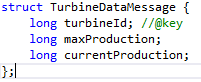
\includegraphics[width=0.3\textwidth,natwidth=250,natheight=200]{turbineDataMessage.PNG} 
	\begin{lstlisting}[language=C++,tabsize=2,basicstyle=\small]
uint_fast32_t DecentralizedParkPilot::regAlgorithm(
	uint_fast32_t globalSetpoint,
	TurbineMessageSeq turbines,
	uint_fast32_t maxProd,
	uint_fast32_t currentProd,
	uint_fast32_t setPoint,
	DDS_SampleInfoSeq turbineInfos,
	uint_fast32_t &cacheCount )
{
	cacheCount = 0;
	if (currentProd >= maxProd)
		return maxProd;

	int availableTurbinesCount = turbines.length();

	for (int i = 0; i < turbines.length(); i++)
	{
		if (!turbineInfos[i].valid_data) {
			availableTurbinesCount--;
			continue;
		}

		if (turbineInfos[i].sample_state == DDS_READ_SAMPLE_STATE) {
			cacheCount++;
		}

		if (turbines[i].currentProduction >= turbines[i].maxProduction)
			availableTurbinesCount--;
	}
	uint_fast32_t localSetpoint = 0;

	if (availableTurbinesCount <= 0)
		localSetpoint = globalSetpoint;
	else
		localSetpoint = globalSetpoint / availableTurbinesCount;

	if (localSetpoint > maxProd) {
		localSetpoint = maxProd;
	}

	return localSetpoint;
}
	\end{lstlisting}
	\captionsetup{format=plain,font=footnotesize,labelfont={bf,defaultCapFont},labelsep=quad,singlelinecheck=no}
	\caption[The regulation algorithm of the decentralized solution]{
		\label{fig:decenRegAlgCode} 
		\footnotesize{%
			Code for the decentralized regulation algorithm used to calculate setpoints.
		}
	}
\end{figure}

\subsection{Cache reads}\label{sec:cachereads}

A cache read happens if the cycle time elapses before all turbine instances have responded with state information, resulting in the same state being read twice. Thus it is a natural result of separating receiving data from the regulation cycle, as done in the decentralized solution. Connext only keeps track of data that has already been read but not how many times that data has been read. Thus a cache read does not include information regarding if the same state has been read multiple times.

The regulation cycle of the decentralized solution does not directly include any communication, thus enabling a significant reduction of regulation cycle time. However, decreasing the cycle time, increases the 'pressure' on Connext by increasing the number of regulation cycles pr. minute, thus increasing the number of states that needs to be published, thus increasing the number of states that needs to be received (assuming that the cycle time of all turbines are equally decreased). This ultimately results in increased number of cache reads and increased network traffic. Thus decreasing the regulation cycle time will increase the number of cache reads.  

Increasing the number of cache reads can be an issue, since it reduces the effectiveness of the regulation cycle. Having a high number of cache reads implies that the regulation has been performed using data used for the previous regulation, thus decreasing the effect of the current regulation.

As a result of this trade-off between reduction in regulation cycle time and number of cache reads, a sleep is introduced at the end of the regulation cycle (as presented in \cref{fig:decenRegCycle}), in order to control the reduction of the regulation cycle. Thus the regulation cycle time is an input parameter of the decentralized solution.

\section{DDS configuration} \label{sec:decen:ddsconf}

The key component used for communication is DDS (see \cref{sec:DSM} for DDS description). This section describes how DDS has been configured for the decentralized solution.

\subsection{Interface Definition Language}\label{sec:decenIdl}

As with the centralized solution, Interface Definition Language (IDL) has been used for generating Data Transfer Objects for the decentralized solution. See centralized IDL \cref{sec:cenIdl} for details.

\begin{figure}[!h]
	\centering
	%	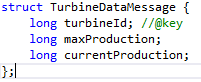
\includegraphics[width=0.3\textwidth,natwidth=250,natheight=200]{turbineDataMessage.PNG} 
	\begin{lstlisting}[language=C++,tabsize=2,basicstyle=\small]
	struct TurbineMessage {
		long turbineId; //@key
		long maxProduction;
		long currentProduction;
		long setPoint;
		long msSinceLastWrite;
		long cacheCount;
	};	
	\end{lstlisting}
	\captionsetup{format=plain,font=footnotesize,labelfont={bf,defaultCapFont},labelsep=quad,singlelinecheck=no}
	\caption[Decentralized turbine message]{
		\label{fig:decenTurbineMessage} 
		\footnotesize{%
			The turbine message .idl file sent from the turbines to all other turbines in the decentralized solution.
		}
	}
\end{figure}

\subsection{Choosing Quality of Service parameters}\label{sec:decenChoosingQoS}

The Quality of Service (QoS) parameters for the decentralized solution is based on the QoS parameters determined for the centralized solution, except for the following key areas:

\begin{description}
	\item[Reliability] of messaging has been changed to best effort messaging in order to reduce the regulation cycle time. This means package drops are allowed for the decentralized solution.
	\item[Durability] of the decentralized solution has been changed to local durability. This means that the current state of every turbine is sent to newly discovered turbines. Note that with best effort messaging there is no guarantee that the states are received, since package drops are allowed. Durability for the regulation cycle has only minor relevance, since newly arrived turbines will receive all states within a short amount of time after being discovered. Thus this setting has only been applied, since an attempt to receive states upon startup is better than receiving no states at all. However, for real life purposes, the turbines should probably be configured with a default setpoint, which is used until data from all turbines has been received, in combination with this setting. 
	\item[Throughput] remains the same as the throughput setting of the centralized solution but for a slightly different reason. New turbine states must be sent as soon as possible, which removes the need for batching. \todo{Hvorfor gør det batching irrelevant?} Thus regular throughput has been chosen for the decentralized solution. 
	\item[Multicast] has been enabled to reduce regulation cycle time and network traffic, as explained in \cref{sec:regCycleChanges}.
\end{description}

\subsection{Detailed quality of service evaluation}

This section provides a detailed evaluation of every parameter used for the decentralized QoS XML. The full QoS XML is presented but only parameter changes from the centralized solution are discussed.

\paragraph{Participant factory} (\cref{fig:decParFacQos}) QoS parameters has been set to be the same as the centralized solution. See Participant factory description of \cref{sec:detailedQoSDesc}.

\begin{figure}[!h]
\begin{lstlisting}[language=XML]
<participant_factory_qos>
	<logging>
		<verbosity>WARNING</verbosity>
		<category>PLATFORM</category>
		<print_format>VERBOSE_TIMESTAMPED</print_format>
		<output_file>ddsadaptor.log</output_file>
	</logging>
</participant_factory_qos>
\end{lstlisting}
\caption[Decentralized participant factory QoS parameters]{
		\label{fig:decParFacQos} 
		\footnotesize{Participant factory QoS parameters of the decentralized solution.}
	}
\end{figure}

\paragraph{Participant} (\cref{fig:decParQos}) QoS parameters has been evaluated as follows (see Participant evaluation of \cref{sec:detailedQoSDesc} for parameters not described):

\begin{itemize}
	\item \textbf{.builtin.multicast\_enabled} value has been set to 1 to enable multicast.
\end{itemize}

\begin{figure}[!h]
\begin{lstlisting}[language=XML]
<participant_qos>
	<participant_name>
		<name>TurbineParticipant</name>
		<role_name>TurbineParticipantRole</role_name>
	</participant_name>
		<database>
		<shutdown_cleanup_period>
			<sec>DURATION_ZERO_SEC</sec>
			<nanosec>1</nanosec>
		</shutdown_cleanup_period>
	</database>
		<transport_builtin>
			<mask>UDPv4</mask>
		</transport_builtin>
	<property>
		<value>
			<element>
				<name>dds.transport.UDPv4.builtin.multicast_enabled</name>
				<value>1</value>
			</element>
			<element>
				<name>dds.transport.UDPv4.builtin.parent.message_size_max</name>
				<value>65535</value>
			</element>
			<element>
				<name>dds.transport.UDPv4.builtin.send_socket_buffer_size </name>
				<value>65535</value>
			</element>
			<element>
				<name>dds.transport.UDPv4.builtin.recv_socket_buffer_size</name>
				<value>2097152</value>
			</element>
		</value>
	</property>
</participant_qos>
\end{lstlisting}
\caption[Decentralized participant QoS parameters]{
		\label{fig:decParQos} 
		\footnotesize{Participant QoS parameters of the decentralized solution.}
	}
\end{figure}

\paragraph{Topic} (\cref{fig:decTopicQos}) QoS parameters are used to initialize DataReader and DataWriter QoS paramters. Thus parameters that applies to both DataReaders and DataWriters have been configured using a Topic profile. Topic QoS parameters have been evaluated as follows:

\begin{itemize}
	\item \textbf{reliability} of the decentralized solution has been set to best effort, as discussed in \cref{sec:decenChoosingQoS}, thus making package drops acceptable.
	\item \textbf{durability} has been set to local durability, thus latest states from all online turbines are sent to newly added turbines.
	
	Note that in combination with best effort reliability, a newly added turbines is not ensured all turbine states. Furthermore the amount of states received from each turbines is the depth value set by the history QoS parameter.
	\item \textbf{history} configures the number of data samples the send and receive buffers can contain on a per instance basis for keyed Topics. With KEEP\_LAST\_HISTORY\_QOS enabled, the latest values of the data samples are kept and old samples are discarded when the limit as set by the depth parameter is reached. Thus the send and receive buffers of the decentralized solution acts like a circular buffer of length 1, meaning, in combination with best effort messaging, only newest states are available to the turbines.
\end{itemize}

\begin{figure}[!h]
\begin{lstlisting}[language=XML]
<topic_qos name="TurbineTopicQos">
	<reliability>
		<kind>DDS_BEST_EFFORT_RELIABILITY_QOS</kind>
	</reliability>
	<durability>
		<kind>TRANSIENT_LOCAL_DURABILITY_QOS</kind>
	</durability>
	<history>
		<kind>KEEP_LAST_HISTORY_QOS</kind>
		<depth>1</depth>
	</history>
</topic_qos>
\end{lstlisting}
\caption[Decentralized Topic QoS parameters]{
		\label{fig:decTopicQos} 
		\footnotesize{Topic QoS parameters of the decentralized solution.}
	}
\end{figure}

\paragraph{DataWriter} (\cref{fig:decDataWriterQos}) QoS parameters has been evaluated as follows (see DataWriter evaluation of \cref{sec:detailedQoSDesc} for parameters not described):

\begin{itemize}
	\item \textbf{lifespan} configures the expiration time of each data sample written by a DataWriter. Thus this parameter is only relevant to DataWriters. Each data sample has an associated expiration time, beyond which the data should not be delivered. Once the sample expires, the data sample will be removed from the DataReaders receive buffers. 
	
	This parameter configures the previously mentioned time limit (\cref{sec:regCycleChanges}) of the decentralized solution. A turbine state expires after 150000000 nanoseconds ($=150$ ms). This value is set after the worst case regulation cycle time of the current Siemens system, to ensure that the decentralized solution do not use data older than what the current Siemens system use for regulation.
	
	Furthermore, this parameter also indirectly controls how many and which turbines should be used for the regulation algorithm. If a state is older than 150 ms, the state is automatically removed from the receive buffer, thus it is removed from the data that is read and used for the regulation algorithm. As the regulation algorithm automatically scales with the number of turbines, from which a state has been received within the latest 150 ms, the turbine which have not sent a new state within 150 ms will be considered offline. For this reason the lifespan parameter is responsible for the tolerance of the decentralized solution. If a turbines fails, the state of the turbine will eventually expire, thus removing the turbine from the regulation algorithm.
\end{itemize}

\begin{figure}[!h]
\begin{lstlisting}[language=XML]
<datawriter_qos>
	<publication_name>
		<name>TurbineDataWriter</name>
	</publication_name>
	<lifespan>
		<duration>
			<sec>0</sec>
			<nanosec>150000000</nanosec>
		</duration>
	</lifespan>
</datawriter_qos>
\end{lstlisting}
\caption[Decentralized DataWriter QoS parameters]{
		\label{fig:decDataWriterQos} 
		\footnotesize{DataWriter QoS parameters of the decentralized solution.}
	}
\end{figure}

\paragraph{DataReader} (\cref{fig:decDataReaderQos}) QoS parameters has been evaluated as follows (see DataReader evaluation of \cref{sec:detailedQoSDesc} for parameters not described):

\begin{itemize}
	\item \textbf{multicast} specifies the multicast addresses on which DataReaders receives data from DataWriters. 
\end{itemize}

\begin{figure}[!h]
\begin{lstlisting}[language=XML]
<datareader_qos>
	<subscription_name>
		<name>TurbineDataReader</name>
	</subscription_name>
	<multicast>
		<kind>AUTOMATIC_TRANSPORT_MULTICAST_QOS</kind>
		<value>
			<element>
				<receive_address>239.192.0.1</receive_address>
			</element>
		</value>
	</multicast>
</datareader_qos>
\end{lstlisting}
\caption[Decentralized DataReader QoS parameters]{
		\label{fig:decDataReaderQos} 
		\footnotesize{DataReader QoS parameters of the decentralized solution.}
	}
\end{figure}